\documentclass{beamer}
\pdfoutput=1

%----------------------------------------------------------------------
% Most users will not need to edit the preamble of the document.
% Instead, skip down to where it says "poster content begins here".
%----------------------------------------------------------------------

\mode<presentation>{\usetheme{poster}}
\usefonttheme{serif}
\setbeamertemplate{bibliography item}{}
\setbeamercolor{bibliography entry author}{fg=black}
\setbeamercolor{bibliography entry title}{fg=black} 
\setbeamercolor{bibliography entry location}{fg=black} 
\setbeamercolor{bibliography entry note}{fg=black}  

\usepackage{amsmath,amssymb,array}
\usepackage{graphicx,tcolorbox}
\usepackage{mathptmx}
\usepackage{multirow}
%\tcbuselibrary{listings,breakable,most,hooks,skins}
\graphicspath{{./graphics/}}
\newcommand{\R}{\mathbb{R}}
\newcommand{\Z}{\mathbb{Z}}
\newcommand{\N}{\mathbb{N}}
\newcommand{\C}{\mathbb{C}}
\newcommand{\Q}{\mathbb{Q}}

\usepackage[orientation=landscape,size=custom,width=121.92,height=91.44,scale=1.2]{beamerposter}
% Note: beamerposter expects measurements in cm
% 121.92cm = 48in, 91.44cm = 36in
% 48x36 inches is standard UIC poster printing size

% Header and footer 
\newcommand{\footleft}{http://mcl.math.uic.edu/}
\newcommand{\footright}{}


%@@@@@@@@@@@@@@@@@@@@@@@@@@@@@@@@@@@@@@@@@@@@@@@@@@@@@@@@@@@@@@@@@@@@@@
%                 POSTER CONTENT BEGINS HERE
%@@@@@@@@@@@@@@@@@@@@@@@@@@@@@@@@@@@@@@@@@@@@@@@@@@@@@@@@@@@@@@@@@@@@@@


\title{Visualizing Elliptic Curves and Their Tori}
\author{Galen Ballew \quad James Duncan}
\institute{University of Illinois at Chicago}

% Main document
\begin{document}
\begin{frame}{}
\begin{columns}[t]
%-- Column 1 ---------------------------------------------------
\begin{column}{0.245\linewidth}

%-- Block 1-1
\begin{block}{Summary}
Our research focuses on elliptic curves $E$ over $\mathbb{Q}$ with complex multiplication (by the maximal order of an imaginary quadratic field). Viewed over $\mathbb{C}$, each $E$ gives rise to two tori, defined by the generators $\omega_1$ and $\omega_2$ of the period lattice. These tori can be constructed virtually into a 3D mesh. Further, this mesh can be translated into gcode and printed using a 3D printer. 
\end{block}

%-- Block 1-2
\begin{block}{Motivation}
Elliptic curves are interesting mathematical pheomena. Certain curves can be used to solve Diophantine equations, part of factoring algorithms, or used in cryptography. Elliptic curves are also a critical element in the proof of Fermat's Last Theorem. This research project is about developing an understanding of elliptic curves, their properties, and creating visualizations of them. 
\end{block}

%-- Block 1-3
\begin{block}{Definition}
An \textbf{elliptic curve}  over a field $K$ of characteristic different than 2 and 3 is 
the geometric locus of an equation of the form
$$E : y^2 = x^3+ax+b,$$
where $a, b \in K$ such that $\Delta := -16 (4 a^3 + 27 b^2) \neq 0$,
together with the projective point ${\cal{O}} =  [0:1:0] \in E(K)$.\\
\\
This equation is called the \textbf{Weierstrass form} of the elliptic curve.
On $E(K)$, the set of points that satisfy $E$, we define a \textbf{group addition law via the chord-tangent method :}\\
\begin{figure}[p]
    \includegraphics[scale=1.2]{PQ}
     \includegraphics[scale=1.2]{2P}
\end{figure}
\end{block} 


\begin{block}{$E$ with coefficients in $\mathbb{Q}$}
Let $E/\Q$ be an elliptic curve, and let $E(\Q)$ be the group of points on $E/\Q$ with rational coefficients. Mordell's theorem states that $E(\Q)$ is a finitely generated abelian group. Then
$$ E(\Q) \simeq \Z^r \oplus E(\Q)_{tors} $$
where $r = r(E)$ is some non-negative integer, called the \textbf{arithmetic rank} of $E/\Q$, and where $E(\Q)_{tors}$ is the group of points of finite order in $E(\Q)$, called the \textbf{torsion subgroup} of $E(\Q)$. 
\end{block}
\end{column}%1

%-- Column 2 ---------------------------------------------------
\begin{column}{0.245\linewidth}

%-- Block 2-1
\begin{block}{$E$ with coefficients in $\mathbb{C}$}
Let $\omega_1$, $\omega_2 \in \mathbb{C}$ such that $\omega_1$ and $\omega_2$ are linearly independent over $\mathbb{R}$. We may then define the complex \textbf{lattice} $\Lambda$ as 
$$ \Lambda = n_1\omega_1 + n_2\omega_2 : n_1, n_2 \in \mathbb{Z} $$

The Weierstrass $\wp$-function is doubly periodic and defined as $$\frac{1}{u^2} + \sum_{\omega \in \Lambda \omega \neq 0} \left( \frac{1}{(u - \omega)^2} - \frac{1}{\omega^2} \right)$$

It also satifies the following differential equation, which is in the form of an elliptic curve $$\wp'(z)^2 = 4\wp(z)^3 - g_2\wp(z) - g_3$$ 
\begin{center}
\includegraphics[width=0.9\columnwidth]{folding}\\
\end{center}

\end{block}

%-- Block 2-2
\begin{block}{Complex Multiplication}
Let $E/\Q$ be an elliptic curve with rational coefficients. We say that $E/\Q$ has \textbf{complex multiplication}, or CM for short, if there is an endomorphism $\phi : E/\Q \rightarrow E/\Q$ that is not a multiplication-by-\textit{n} map for any integer $n$, so that $\Z \subsetneq$ End($E$). 
There are 9 curves, up to isomorphism, with CM by the maximal order of an imaginary quadratic field and they are the focus of our research. 
  \begin{center}
    \begin{tabular}{ | c | c | } \hline
    \emph{ Cremona Label} & \emph{Equation} \\ \hline
 64a4 & $y^2 = x^3 + x$ \\ \hline
256a1 &$y^2 = x^3 + 4x^2 + 2x$ \\ \hline 
27a3 & $y^2 + y = x^3$ \\ \hline
49a1&$y^2 + xy = x^3 - x^2 - 2x -1$ \\ \hline
121b1 &  $y^2 + y = x^3 - x^2 - 7x + 10$ \\ \hline
361a1 & $y^2 + y = x^3 - 38x + 90$ \\ \hline
1849a1 & $y^2 + y = x^3 - 860x^2 + 9707$ \\ \hline
4489a1 & $y^2 + y = x^3 - 7370x^2 + 243528$ \\ \hline
26569a1 & $y^2 + y = x^3 - 2174420x + 1234136692$ \\ \hline
    \end{tabular}
  \end{center}

\vspace{0.05em}

\begin{center}
% Two copies of a placeholder picture.
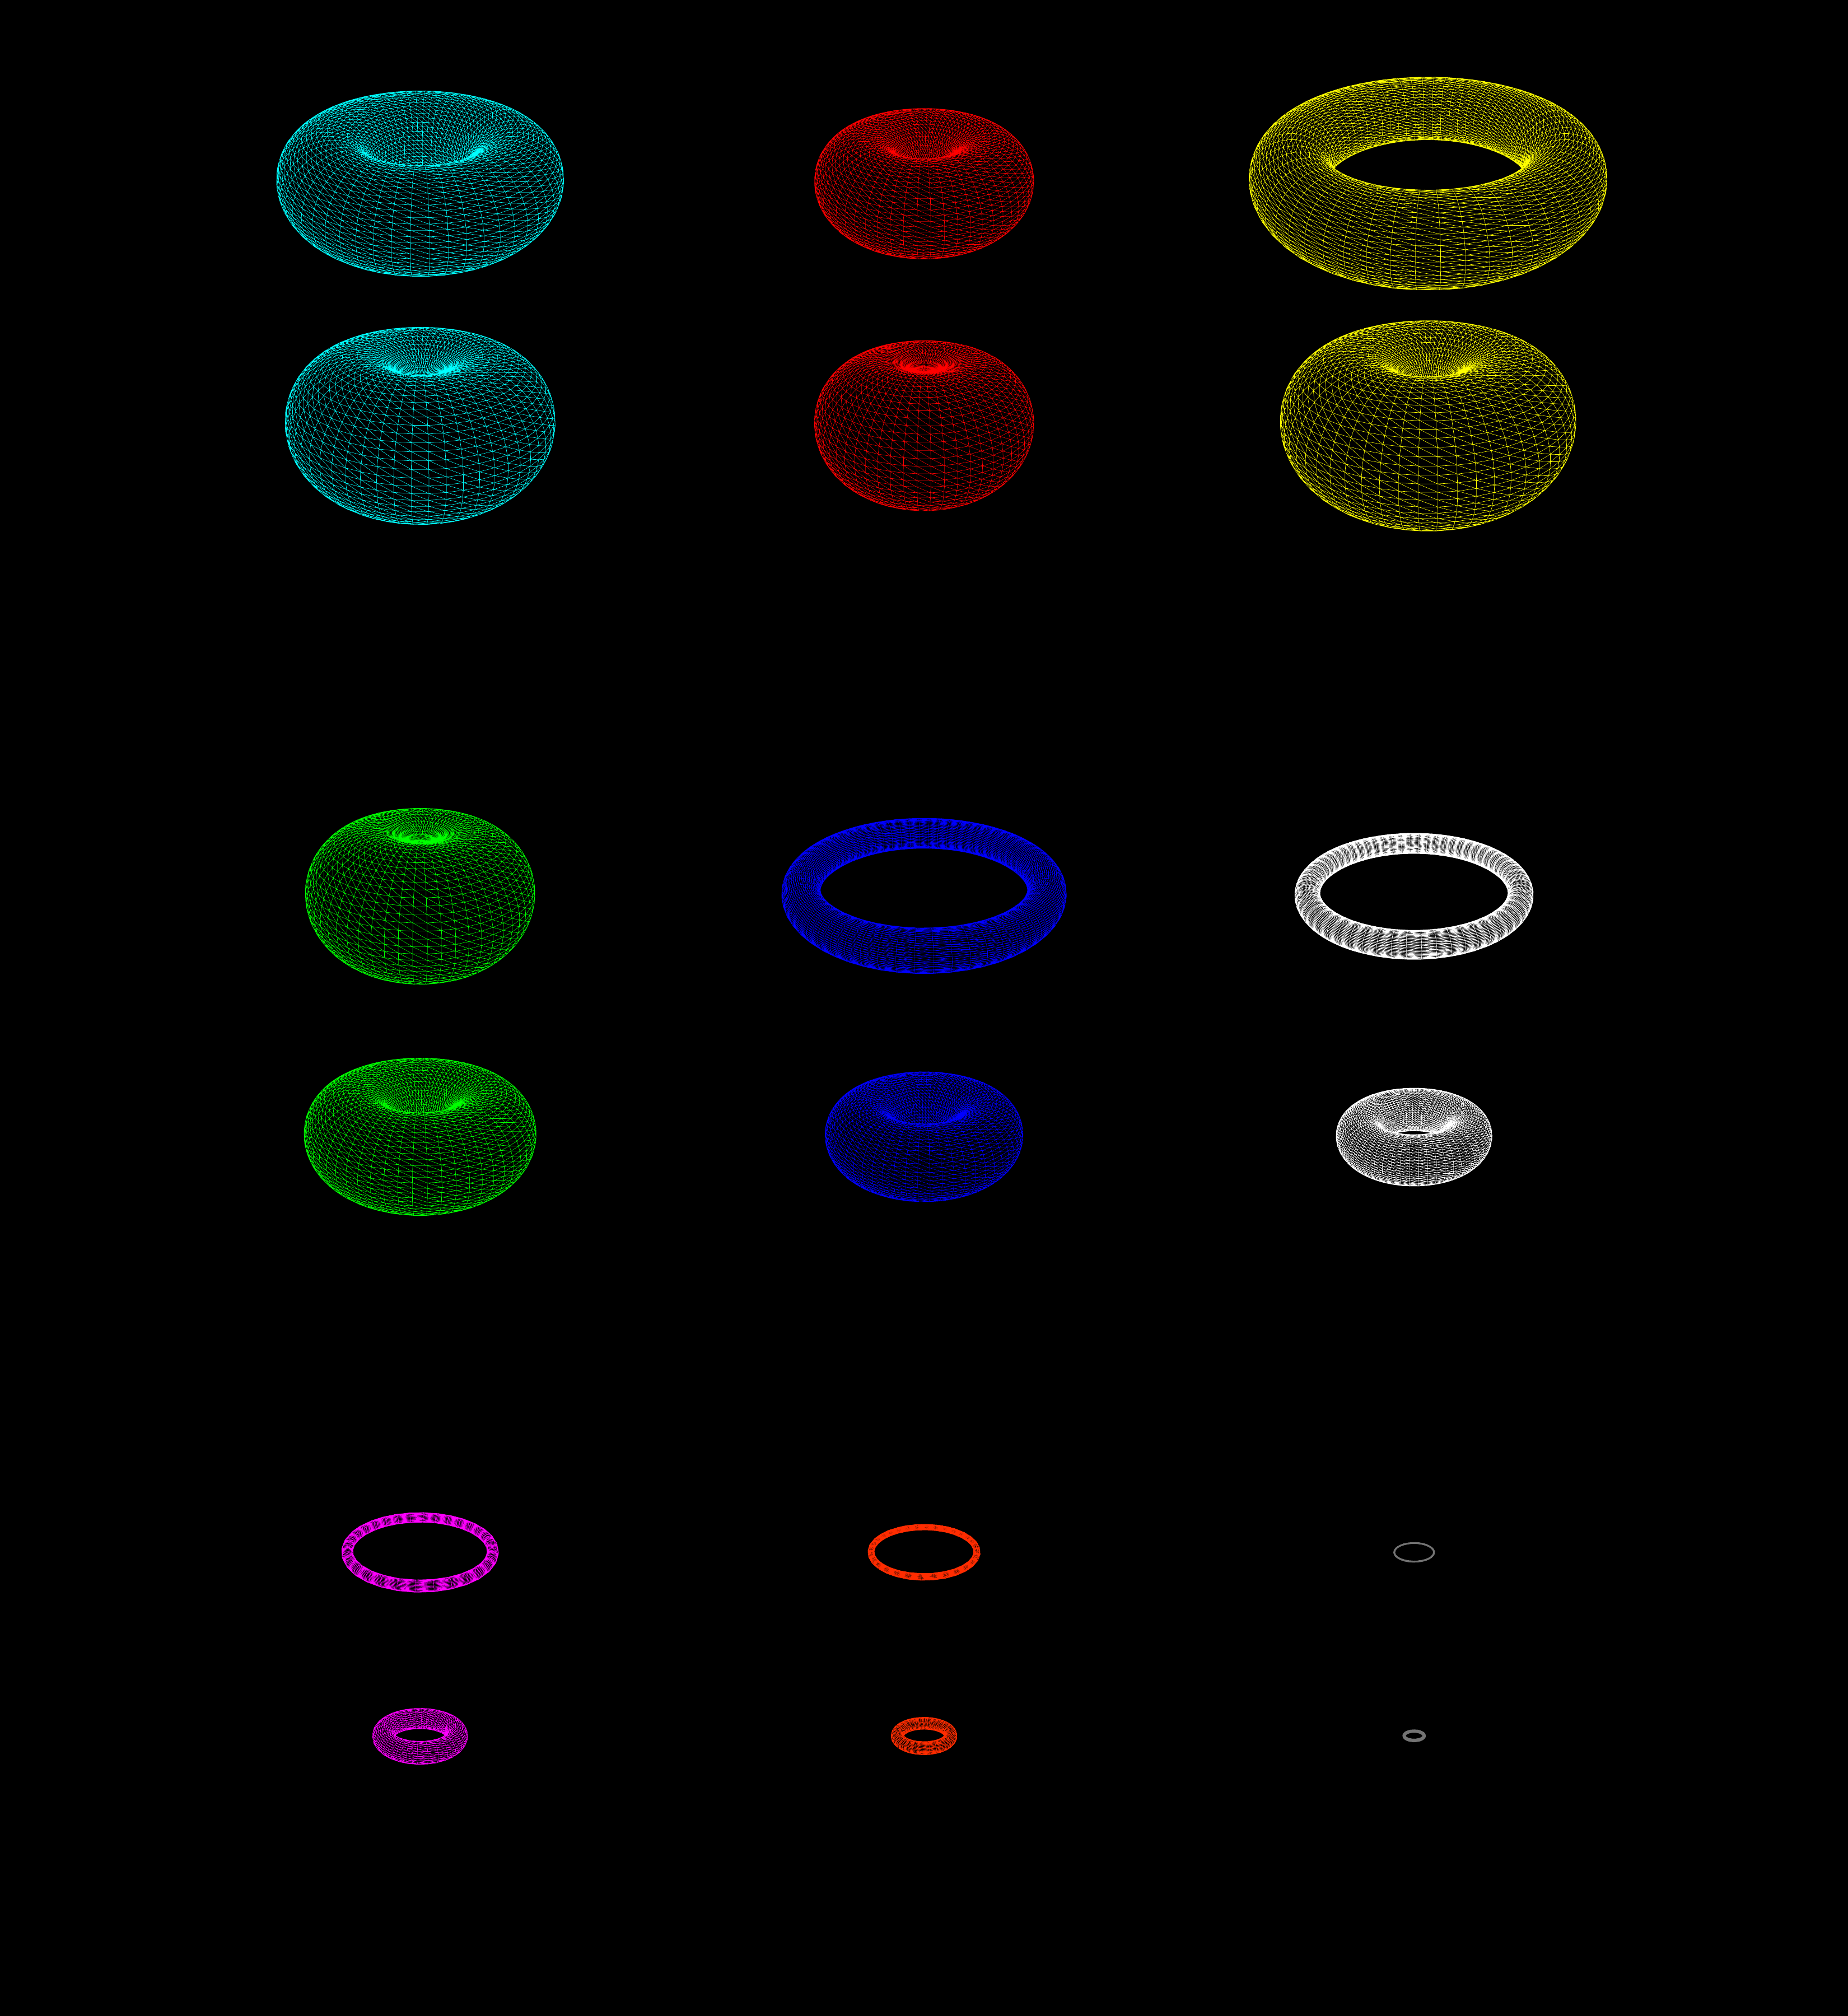
\includegraphics[width=0.9\columnwidth]{curves}\\
\end{center}
\end{block}
\end{column}%2


%-- Column 3 ---------------------------------------------------
\begin{column}{0.245\linewidth}

\begin{block}{Sample SAGE Code}
SAGE was used to calculate the period lattice of each curve, which gives the basis that defines their tori. The periods were calculated to an arbitrary precision using Gauss's Arithmetic-Geometric Mean. Further, SAGE was used to compile characteristic information about the curves, as seen in the table below. 
\begin{center}
\includegraphics[width=0.9\columnwidth]{code}
\end{center}
\end{block}

%%%
\begin{block}{Curve Datum}
  \begin{center}
    \begin{tabular}{ | c | c | c | c | c | c | c | } \hline
      \emph{Label} & \emph{Discriminant} & \emph{Conductor} & \emph{Torsion} & \emph{Rank} & \emph{CM Field} \\ \hline\hline

      \multirow{2}{*}{ 64a4 } & -64 & 64 & $\Z/2$ & 0 & $\Q(\sqrt{-1})$ \\ \cline{2-6} % 1
      \multirow{2}{*}{} & \multicolumn{5}{ c |}{$j$-invariant: 1728} \\ \hline\hline

      \multirow{2}{*}{ 256a1 } & 512 & 256 & $\Z/2$ & 1 & $\Q(\sqrt{-2})$ \\ \cline{2-6} % 2
      \multirow{2}{*}{} & \multicolumn{5}{ c |}{$j$-invariant: 8000} \\ \hline\hline

      \multirow{2}{*}{ 27a3 } & -27 & 27 & $\Z/3$ & 0 & $\Q(\sqrt{-3})$ \\ \cline{2-6} % 3
      \multirow{2}{*}{} & \multicolumn{5}{ c |}{$j$-invariant: 0} \\ \hline\hline

      \multirow{2}{*}{ 49a1 } & -343 & 49 & $\Z/2$ & 0 & $\Q(\sqrt{-7})$ \\ \cline{2-6} % 4
      \multirow{2}{*}{} & \multicolumn{5}{ c |}{$j$-invariant: -3375} \\ \hline\hline

      \multirow{2}{*}{ 121b1 } & -1331 & 121 & Trivial & 1 & $\Q(\sqrt{-11})$ \\ \cline{2-6} % 5
      \multirow{2}{*}{} & \multicolumn{5}{ c |}{$j$-invariant: -32768} \\ \hline\hline

      \multirow{2}{*}{ 361a1 } & -6859 & 361 & Trivial & 1 & $\Q(\sqrt{-19})$ \\ \cline{2-6} % 6
      \multirow{2}{*}{} & \multicolumn{5}{ c |}{$j$-invariant: -884736} \\ \hline\hline

      \multirow{2}{*}{ 1849a1 } & -79507 & 1849 & Trivial & 1 & $\Q(\sqrt{-43})$ \\ \cline{2-6} % 7
      \multirow{2}{*}{} & \multicolumn{5}{ c |}{$j$-invariant: -884736000} \\ \hline\hline

      \multirow{2}{*}{ 4489a1 } & -300763 & 4489 & Trivial & 1 & $\Q(\sqrt{-67})$ \\ \cline{2-6} % 8
      \multirow{2}{*}{} & \multicolumn{5}{ c |}{$j$-invariant: -14719795200} \\ \hline\hline

      \multirow{2}{*}{ 26569a1 } & -4330747 & 26569 & Trivial & 1 & $\Q(\sqrt{-163})$ \\ \cline{2-6} % 9
      \multirow{2}{*}{} & \multicolumn{5}{ c |}{$j$-invariant: -262537412640768000} \\ \hline
    \end{tabular}
  \end{center}
\end{block}

%-- Block 3-3
\begin{block}{Mesh Building}
The images of the tori are wireframe renderings of their virtual 3-dimensional meshes. These were constructed in Blender and Autodesk Maya. All of the tori were built and visualized using relative scale. The meshes are the basis for the 3D prints. They were exported as .stl or .obj and imported into Cura for the Ultimaker2 3D printer. 
\end{block}




\end{column}%3


%-- Column 4 ---------------------------------------------------
\begin{column}{0.245\linewidth}

%-- Block 4-1

\begin{block}{Tori Visualization}
\vspace{0.5em}

\begin{center}
% THREE copies of a placeholder picture.
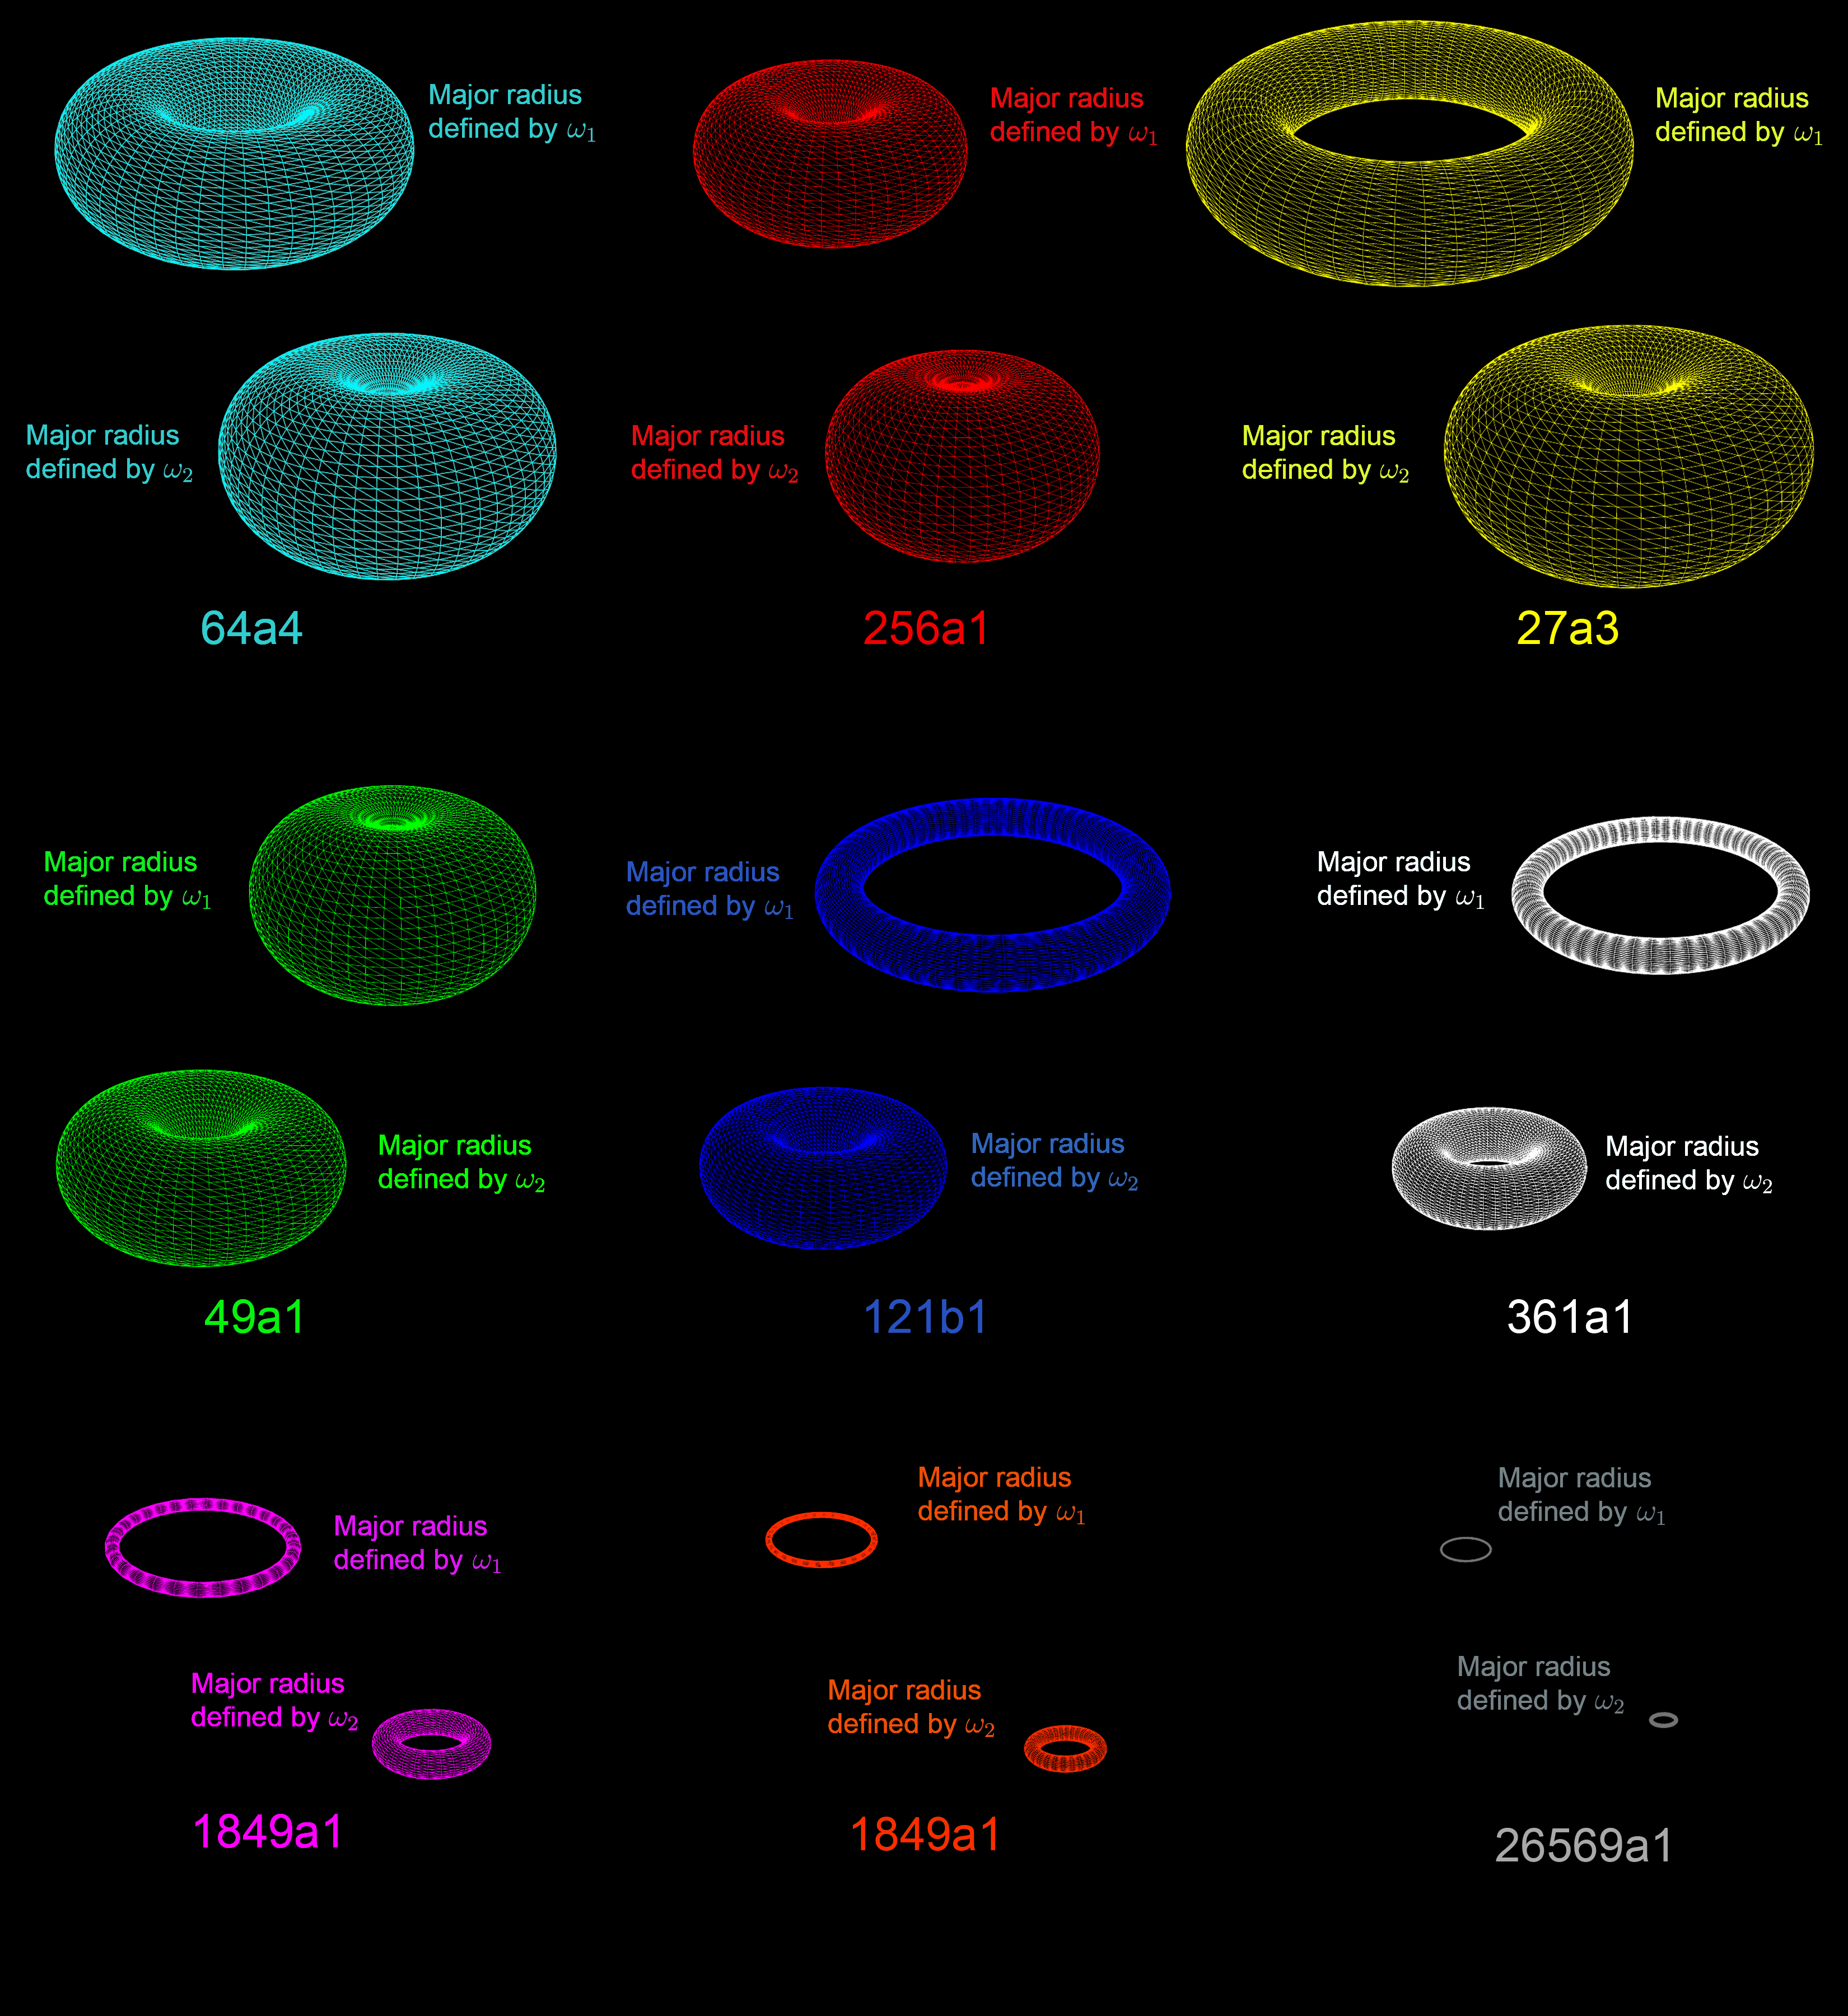
\includegraphics[width=0.9\columnwidth]{tori}\\[1em]

\end{center}
\end{block}


%-- Block 4-2
\begin{block}{3D Printing}
The Cura software converts 3D meshes into G-code. G-code is a programming language for machine tools. It converts the 3D mesh into (X,Y,Z) coordinates for the printhead of the Ultimaker2. 
\begin{center}
\includegraphics[scale = 0.25]{printing}
\end{center}
\end{block}

%-- Block 4-3
\begin{block}{Future Research}
There is currently no definitive method for calculating the rank of an elliptic curve. More specifically, it is unknown whether the rank of an elliptic curve can be arbitrarily large (i.e. whether ranks are bounded or unbounded.) Currently, the largest known rank is \textit{at least} 24, discovered by Martin and McMillen in 2000. 
\end{block}

%-- Block 4-4
\begin{block}{References}
\begin{thebibliography}{99}
\bibitem{cojocaru} A.C. Cojocaru. \emph{Primes, Elliptic Curves, and Cyclic Groups: A Synopsis}. (2016)
\bibitem{silverman}    J. Siverman, J. Tate. \emph{Rational Points on Elliptic Curves}. Undergraduate Texts in Mathematics (2015)
\end{thebibliography}
\end{block}
\end{column}%4

\end{columns}
\end{frame}
\end{document}
